%!TEX program = lualatex
\documentclass[11pt]{article}
\usepackage[a4paper, margin=1in, includehead]{geometry}
\geometry{a4paper} 
\usepackage[table, svgnames, dvipsnames]{xcolor}
\usepackage{makecell, cellspace, caption}
\usepackage[utf8]{inputenc}
\usepackage{textcomp}
\usepackage[most]{tcolorbox}
\usepackage{enumitem}
\usepackage{multicol}
\usepackage{graphicx} 
\usepackage{titling}
\usepackage{fancyhdr}
\usepackage{tabularray}
\pagestyle{fancy}
\fancyhf{}
\fancyhfoffset[L]{1cm} % left extra length
\fancyhfoffset[R]{1cm} % right extra length
\rhead{\textbf{\textit{Page-\thepage}}}
\lhead{\textbf{\textit{Test Document for PedalPal}}}
\cfoot{}
\usepackage{amsmath,amssymb}  
\usepackage{bm}  
\usepackage[pdftex,bookmarks,colorlinks,breaklinks]{hyperref}  
\hypersetup{linkcolor=black,citecolor=black,filecolor=black,urlcolor=blue} % black links, for printed output
\usepackage{memhfixc} 
\usepackage{pdfsync}  
\usepackage{fancyhdr}
\usepackage{lmodern}
\usepackage{wrapfig}
\usepackage[page,toc,titletoc,title]{appendix}

\usepackage{fontspec}
\setmainfont{Arial}

\pagestyle{fancy}

\usepackage{titlesec}
\begin{document}
\begin{titlingpage}
\begin{flushright}
    \rule{16cm}{5pt}\vskip1cm
    \textbf{{\fontsize{30}{36}\selectfont Test Document}\\ \vspace{1cm}\huge{for}\\\vspace{1cm}\Huge{PedalPal}\\ \vspace{1.5cm}\LARGE{Version 1.0}\\\vspace{1cm}\LARGE{Prepared by}}
\end{flushright}
\vspace{1.0cm}
\large{\begin{tabular*}{\columnwidth}{@{\extracolsep{\stretch{1}}}*{3}{c}@{}}
    \Large{\textbf{Group \# 4}} & & \Large{\textbf{Group Name: Bit Brewers}} \\
    \\
    \textbf{Raghav Manglik} & \textbf{220854} & \href{mailto:raghavkmanglik@gmail.com}{raghavkmanglik@gmail.com} \\
    \textbf{Amogh Bhagwat} & \textbf{220288} & \href{mailto:amogh.2004b@gmail.com}{amogh.2004b@gmail.com} \\
    \textbf{Srishti Chandra} & \textbf{221088} & \href{mailto:chandra.srishti2403@gmail.com}{chandra.srishti2403@gmail.com} \\
    \textbf{Wadkar Srujan Nitin} & \textbf{221212} & \href{mailto:srujanwadkar@gmail.com}{srujanwadkar@gmail.com} \\
    \textbf{Anaswar K B} & \textbf{220138} & \href{mailto:anaswarkb013@gmail.com}{anaswarkb013@gmail.com} \\
    \textbf{Khushi Gupta} & \textbf{220531} & \href{mailto:khushi07g@gmail.com}{khushi07g@gmail.com} \\
    \textbf{Ananya Singh Baghel} & \textbf{220136} & \href{mailto:ananyabaghel2004@gmail.com}{ananyabaghel2004@gmail.com} \\
    \textbf{Pathe Nevish Ashok} & \textbf{220757} & \href{mailto:nevu.pathe1234@gmail.com}{nevu.pathe1234@gmail.com} \\
    \textbf{Debraj Karmakar} & \textbf{220329} & \href{mailto:debraj2003jsr@gmail.com}{debraj2003jsr@gmail.com} \\
    \textbf{Kaneez Fatima} & \textbf{220496} & \href{mailto:kaneezfatimamehdi7@gmail.com}{kaneezfatimamehdi7@gmail.com} \\
    
\end{tabular*}}

\vspace{1.5cm}
\begin{center}
\large{
\begin{tabular}{l l}
    \textbf{Course:} & \textbf{CS253} \\
    \textbf{Mentor TA:} & \textbf{Mr. Bharat} \\
    \textbf{Instructor:} & \textbf{Prof. Indranil Saha} \\
    \textbf{Date:} & \textbf{January 25, 2024}
\end{tabular}
}
\end{center}
\end{titlingpage}

\titleformat{name=\section}[block]
  {\sffamily\LARGE}
  {}
  {0pt}
  {\colorsectionx}
\titlespacing*{\section}{0pt}{\baselineskip}{\baselineskip}
\newcommand{\colorsectionx}[1]{\colorbox{gray!120}{\parbox{\dimexpr\textwidth-2\fboxsep}{\color{white} \centering \huge{\textbf{Contents}}}}}

\tableofcontents

\newpage
\titleformat{name=\section}[block]
  {\sffamily\LARGE}
  {}
  {0pt}
  {\colorsection}
\titlespacing*{\section}{0pt}{\baselineskip}{\baselineskip}

\newcommand{\colorsection}[1]{\colorbox{gray!120}{\parbox{\dimexpr\textwidth-2\fboxsep}{\color{white}\huge{\textbf\thesection. }\ #1}}}

\section{\centering{\textbf{Revisions}}}
\begin{center}
\begin{tabular}{|c|c|c|c|}
    \hline
    \rowcolor{Gainsboro!60}
    \textbf{Version} & \textbf{Primary Author(s)} & \textbf{Description of Version} & \textbf{Date Completed} \\
    \hline
    \makecell{v1.0} & \makecell{Raghav Manglik \\ Amogh Bhagwat \\ Srishti Chandra \\ Wadkar Srujan Nitin \\ Pathe Nevish Ashok \\ Debraj Karmakar \\ Khushi Gupta \\ Ananya Baghel \\ Anaswar K B \\ Kaneez Fatima \\} & \makecell{First version of the \\ Test Document} & \makecell{29/03/24} \\
    \hline
\end{tabular}
\end{center}

\newpage
\section{\centering{\textbf{Introduction}}}

\newpage
\section{\centering{\textbf{Unit Testing}}}
\subsection{Authentication}
\subsubsection{Registering a User}
\textbf{API Endpoint: } \texttt{/auth/register/} \\
\textbf{Test Owner: } Amogh Bhagwat \\
\textbf{Date: } 25/03/2024 \\
\textbf{Test Description: } This test case is used to check if a user can register successfully. \\
\textbf{Test Results: } User is able to register successfully. If a user with the email already exists, appropriate error message is shown. Authentication token is also generated correctly. \\
\begin{center}
    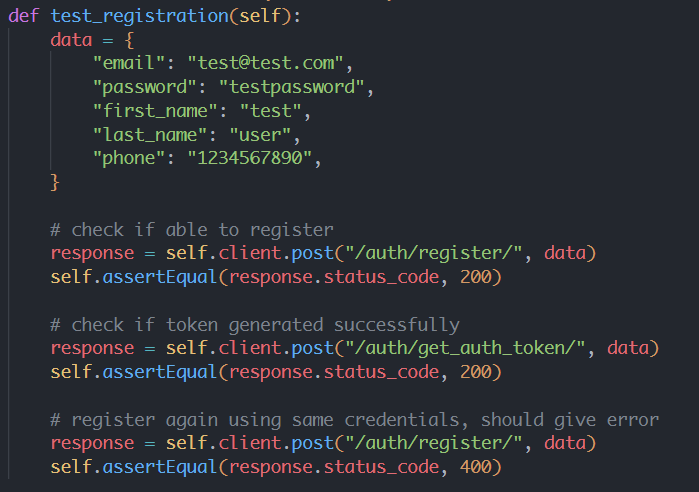
\includegraphics[scale=0.8]{unit_testing_codes/register.png}
\end{center}

\subsubsection{Logging in a User}
\textbf{API Endpoint: } \texttt{/auth/login/} \\
\textbf{Test Owner: } Amogh Bhagwat \\
\textbf{Date: } 25/03/2024 \\
\textbf{Test Description: } This test case is used to check if a user can login successfully. \\
\textbf{Test Results: } User is able to login successfully. If the user enters wrong password or the user does not exist, appropriate error message is shown. \\

\begin{center}
    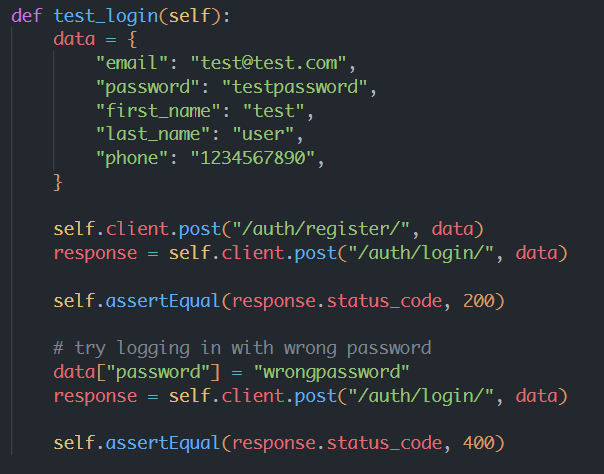
\includegraphics[scale=0.7]{unit_testing_codes/login.png}
\end{center}

\subsubsection{Email Verification}
\textbf{API Endpoint: } \texttt{/auth/verify/} \\
\textbf{Test Owner: } Amogh Bhagwat \\
\textbf{Date: } 25/03/2024 \\
\textbf{Test Description: } This test case is used to check if a user can verify their email successfully. \\
\textbf{Test Results: } User receives the mail containing the link to verify their email successfully. On clicking the link, their email is verified. If the OTP in the link is modified, the verification fails. \\

\begin{center}
    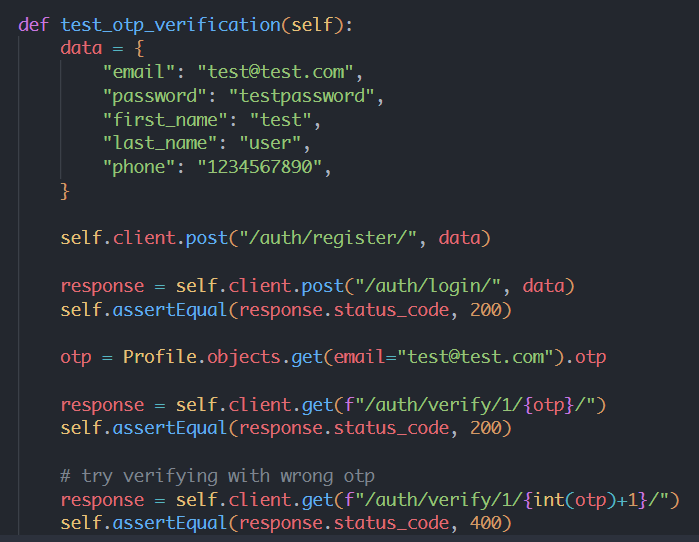
\includegraphics[scale=0.6]{unit_testing_codes/verify.png}
\end{center}

\subsection{Cycle Bookings}
\subsubsection{Starting Ride Instantly}
\textbf{API Endpoint: } \texttt{/booking/book/} \\
\textbf{Test Owner: } Khushi Gupta \\
\textbf{Date: } 26/03/2024 \\
\textbf{Test Description: } This test case is used to check if a user can start a ride instantly by scanning the QR code on the lock. \\
\textbf{Test Results: } User is able to start the ride instantly by scanning the QR code on the lock. The following edge cases were tested - 
\begin{itemize}
    \itemsep 0em
    \item If the user has negative balance in their wallet, they are denied to start the ride.
    \item If the QR code is invalid, appropriate error message is shown.
    \item If the lock has no cycle attached to it, appropriate message is shown.
    \item If the user already has an active ride in progress, they are denied to start another ride.
    \item If the cycle is already booked by some other user, appropriate message is shown.
\end{itemize}
The test database is initialized as follows
\begin{center}
    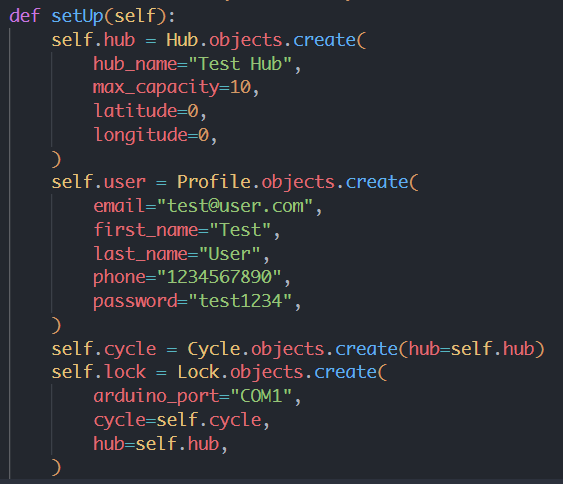
\includegraphics[scale=0.6]{unit_testing_codes/start_ride_setup.png}
\end{center}
The edge cases are tested as follows
\begin{center}
    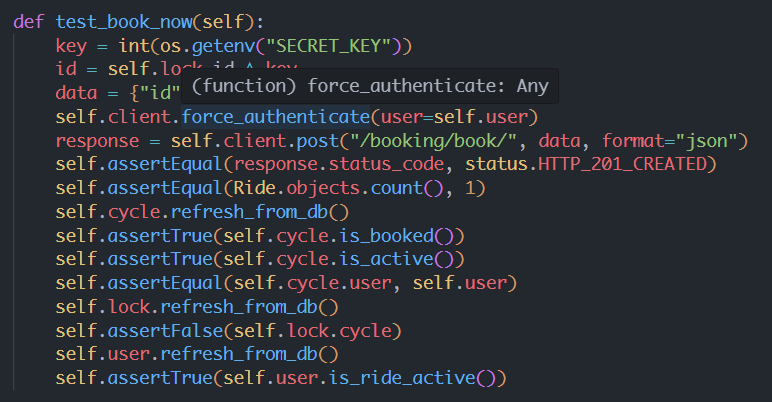
\includegraphics[scale=0.5]{unit_testing_codes/start_ride_1.png}\\
    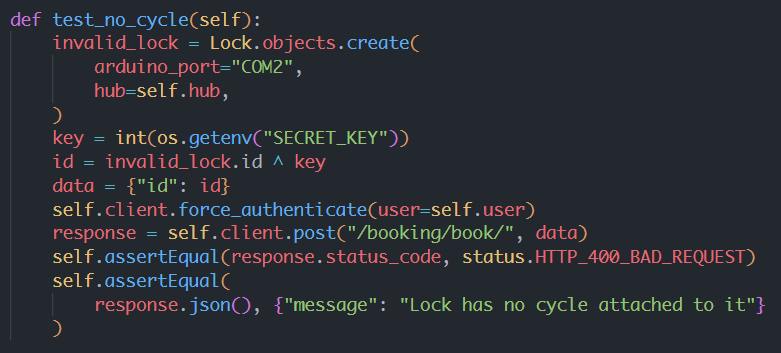
\includegraphics[scale=0.7]{unit_testing_codes/start_ride_2.png}\\
    Lock has no cycle attached to it\\
    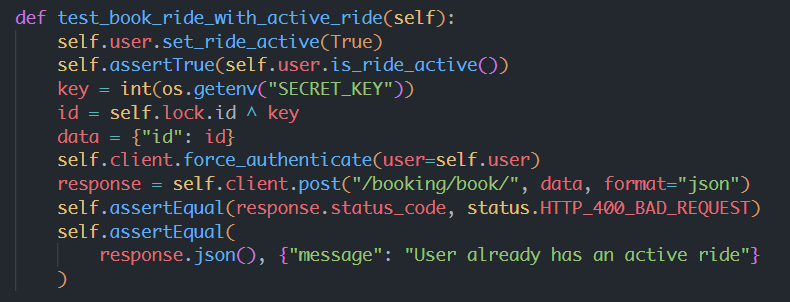
\includegraphics[scale=0.7]{unit_testing_codes/start_ride_3.png}\\
    User already has an active ride\\
    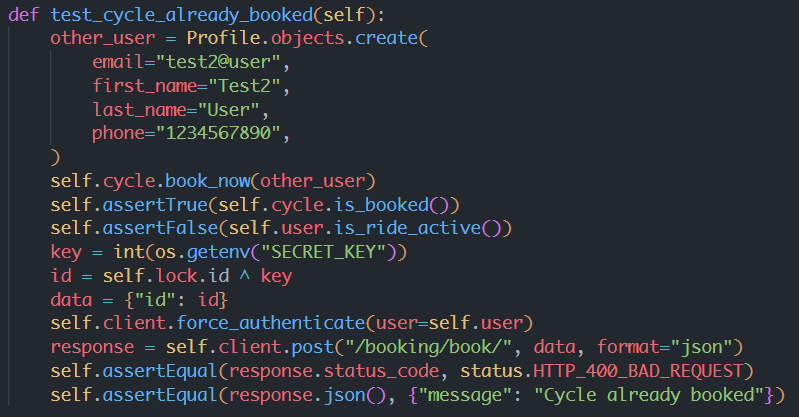
\includegraphics[scale=0.7]{unit_testing_codes/start_ride_4.png}\\
    Cycle is already booked by another user\\
    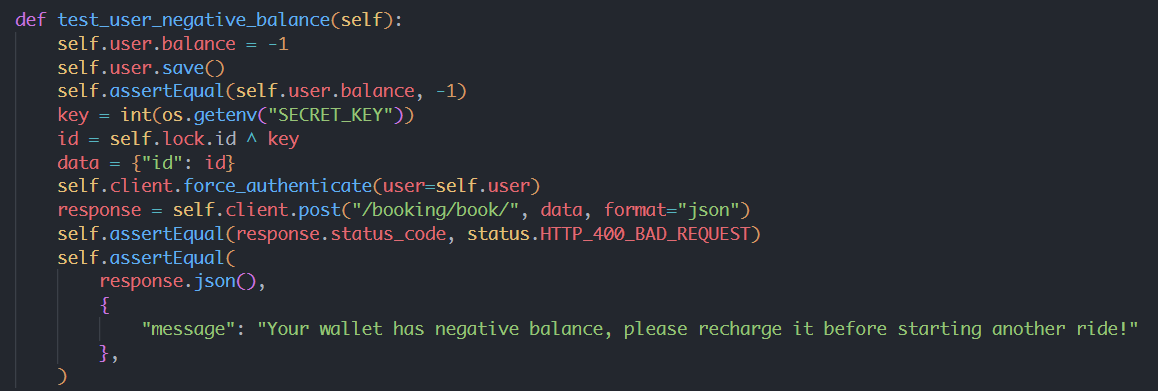
\includegraphics[scale=0.5]{unit_testing_codes/start_ride_5.png}
    User has negative balance in their wallet
\end{center}


\subsubsection{Ending Ride}
\textbf{API Endpoint: } \texttt{/booking/end/} \\
\textbf{Test Owner: } Khushi Gupta \\
\textbf{Date: } 26/03/2024 \\
\textbf{Test Description: } This test case is used to check if a user can end a ride successfully. \\
\textbf{Test Results: } User is able to end the ride successfully by scanning the QR code on the lock. The following edge cases were tested -
\begin{itemize}
    \itemsep 0em
    \item If the QR code is invalid, appropriate error message is shown.
    \item If the lock is already attached to another cycle, appropriate message is shown.
    \item If the user does not have an active ride, appropriate message is shown.
\end{itemize}

The test database is initialized as follows
\begin{center}
    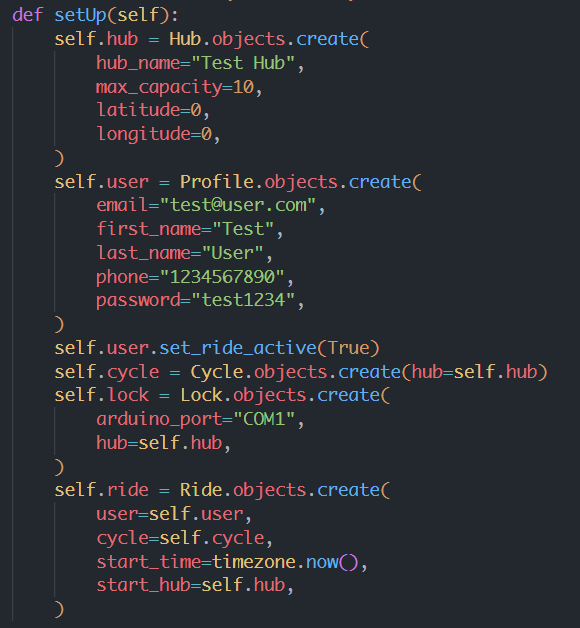
\includegraphics[scale=0.6]{unit_testing_codes/end_ride_setup.png}
\end{center}

The edge cases are tested as follows
\begin{center}
    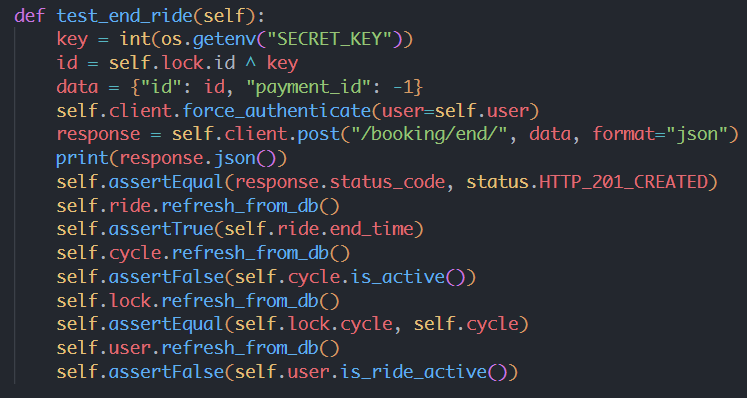
\includegraphics[scale=0.75]{unit_testing_codes/end_ride_1.png}\\
    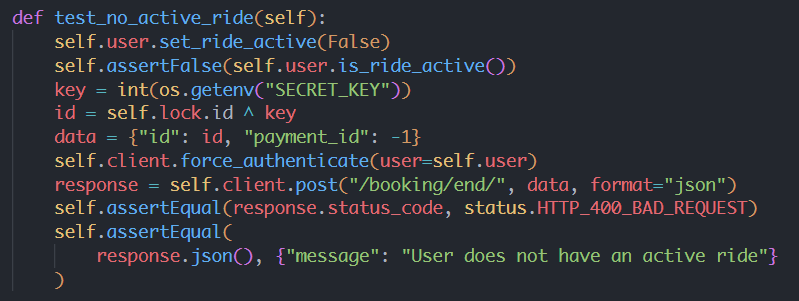
\includegraphics[scale=0.7]{unit_testing_codes/end_ride_2.png}\\
    User does not have an active ride\\
    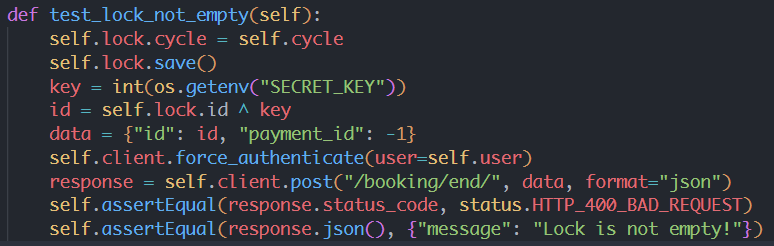
\includegraphics[scale=0.72]{unit_testing_codes/end_ride_3.png}\\
    Lock is already attached to another cycle\\
\end{center}

\subsubsection{Booking a Cycle for Later}
\textbf{API Endpoint: } \texttt{/booking/book\_later/} \\
\textbf{Test Owner: } Nevish Pathe \\
\textbf{Date: } 26/03/2024 \\
\textbf{Test Description: } This test case is used to check if a subscribed user can book a cycle for later. \\
\textbf{Test Results: } User is able to book a cycle for later successfully. The following edge cases were tested -
\begin{itemize}
    \itemsep 0em
    \item If the user has insuffienct balance in their wallet, they are denied to book a cycle.
    \item If the user has not subscribed to the service, they are denied to book a cycle for later.
    \item If the desired cycle is already booked by some other user, appropriate message is shown.
    \item If the desired start time is in the past, appropriate message is shown.
    \item If there is no cycle available at the desired hub, appropriate message is shown.
\end{itemize}

The test database is initialized as follows
\begin{center}
    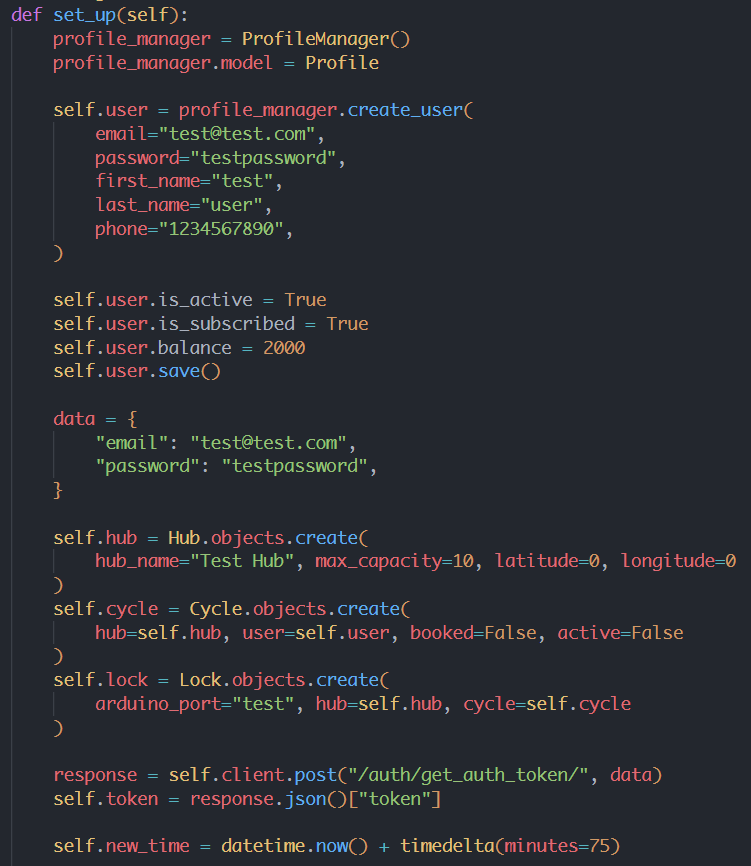
\includegraphics[scale=0.75]{unit_testing_codes/book_later_setup.png}
\end{center}

The edge cases are tested as follows

\begin{center}
    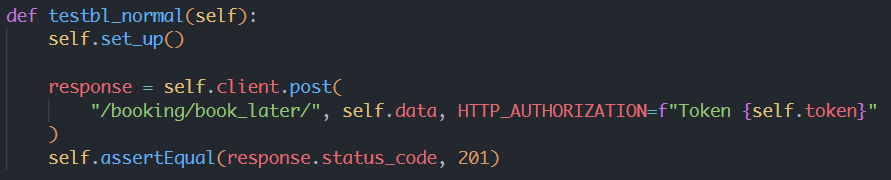
\includegraphics[scale=0.7]{unit_testing_codes/book_later_1.png}\\
    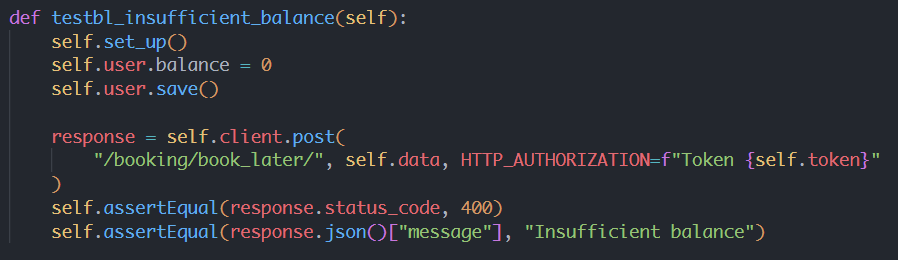
\includegraphics[scale=0.7]{unit_testing_codes/book_later_2.png}\\
    User has insufficient balance in their wallet\\
    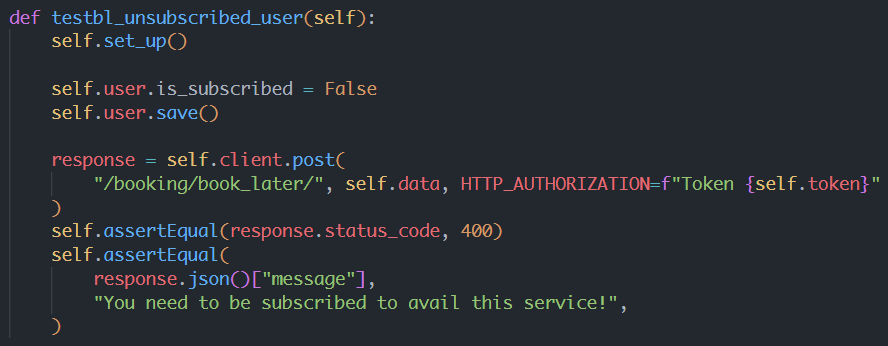
\includegraphics[scale=0.7]{unit_testing_codes/book_later_3.png}\\
    User has not subscribed to the service\\
    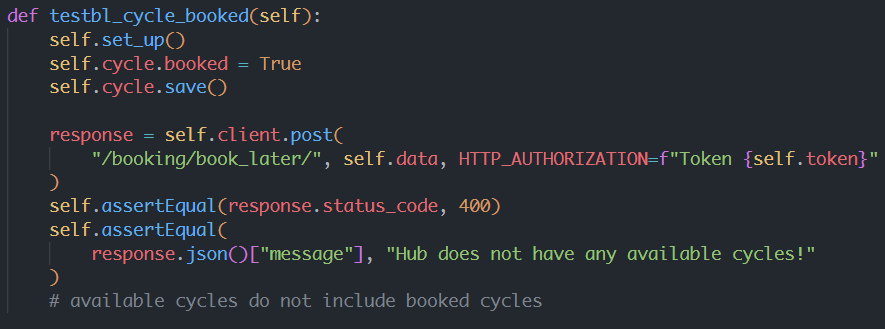
\includegraphics[scale=0.7]{unit_testing_codes/book_later_4.png}\\
    Cycle is already booked by another user\\
    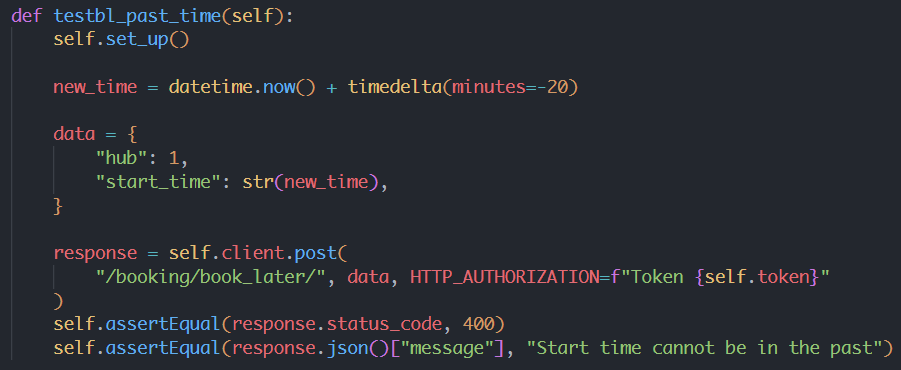
\includegraphics[scale=0.6]{unit_testing_codes/book_later_5.png}\\
    Desired start time is in the past\\
    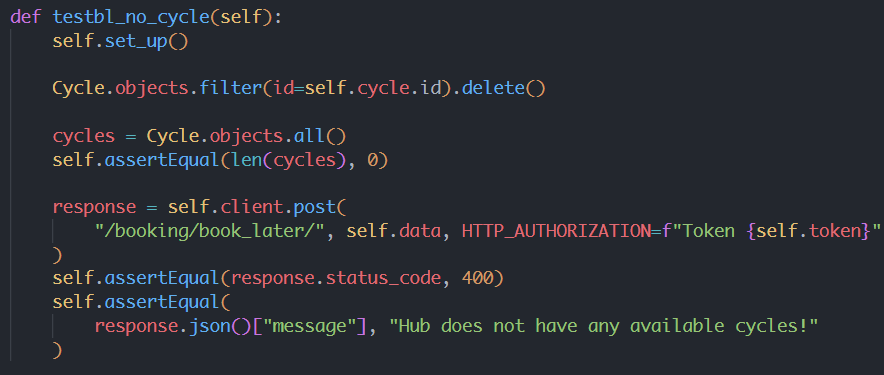
\includegraphics[scale=0.6]{unit_testing_codes/book_later_6.png}\\
    No cycle available at the desired hub\\
\end{center}

\subsubsection{Getting Details of Each Hub}
\textbf{API Endpoint: } \texttt{/booking/view\_hubs/} \\
\textbf{Test Owner: } Nevish Pathe \\
\textbf{Date: } 26/03/2024 \\
\textbf{Test Description: } This test case is used to check if a user can get the details of each hub. \\
\textbf{Test Results: } User is able to get the details of each hub successfully.\\
The database is pre-populated with various hub details in the \texttt{setUp()} method.

\begin{center}
    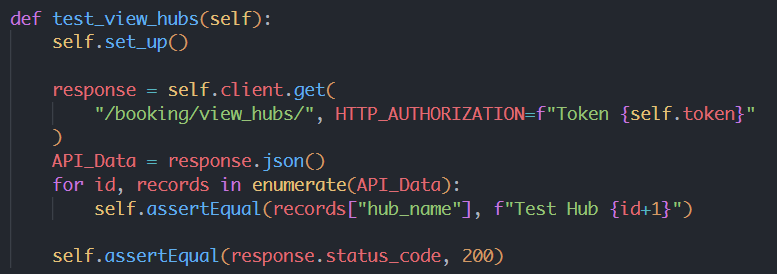
\includegraphics[scale=0.7]{unit_testing_codes/view_hubs.png}
\end{center}

\subsection{User Analytics}
\subsubsection{Viewing Ride History}
\textbf{API Endpoint: } \texttt{/analytics/history/} \\
\textbf{Test Owner: } Kaneez Fatima \\
\textbf{Date: } 25/03/2024 \\
\textbf{Test Description: } This test case is used to check if a user can view their ride history. \\
\textbf{Test Results: } User is able to view their ride history successfully.\\
The database is initialized with multiple rides in the \texttt{setUp()} method.
\begin{center}
    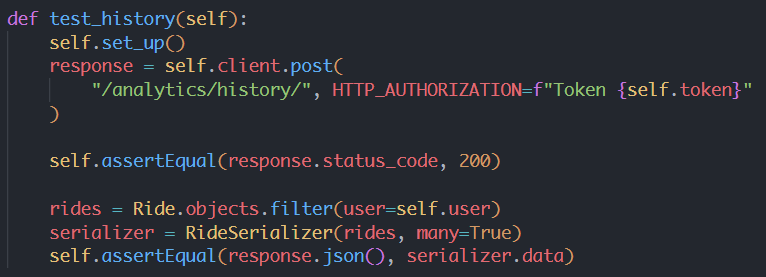
\includegraphics[scale=0.8]{unit_testing_codes/ride_history.png}
\end{center}

\subsubsection{Viewing Past Bookings}
\textbf{API Endpoint: } \texttt{/analytics/booking\_history/} \\
\textbf{Test Owner: } Kaneez Fatima \\
\textbf{Date: } 25/03/2024 \\
\textbf{Test Description: } This test case is used to check if a user can view their past and active bookings. \\
\textbf{Test Results: } User is able to view their past bookings successfully.\\
The database is initialized with multiple bookings in the \texttt{setUp()} method.
\begin{center}
    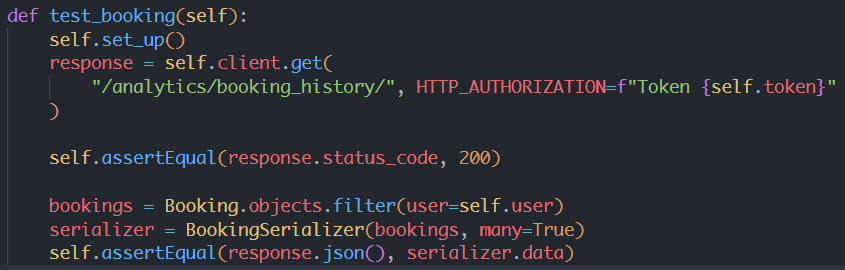
\includegraphics[scale=0.7]{unit_testing_codes/booking_history.png}
\end{center}

\subsection{Maintenance}
\subsubsection{Reporting an Issue}
\textbf{API Endpoint: } \texttt{/maintenance/feedbacks/add/} \\
\textbf{Test Owner: } Ananya Baghel \\
\textbf{Date: } 28/03/2024 \\
\textbf{Test Description: } This test case is used to check if a user can report an issue with the cycle. \\
\textbf{Test Results: } User is able to report an issue with the cycle successfully.\\

\begin{center}
    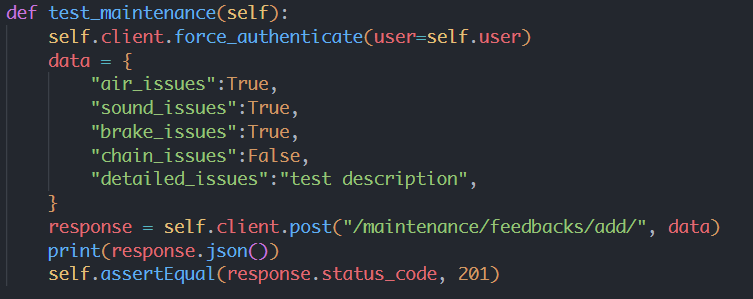
\includegraphics[scale=0.7]{unit_testing_codes/report_issue.png}
\end{center}

\subsection{Payment}
\subsubsection{Getting Wallet Balance}
\textbf{API Endpoint: } \texttt{/payment/get\_balance/} \\
\textbf{Test Owner: } Ananya Baghel \\
\textbf{Date: } 28/03/2024 \\
\textbf{Test Description: } This test case is used to check if a user can get their wallet balance. \\
\textbf{Test Results: } User is able to get their wallet balance successfully.\\

\begin{center}
    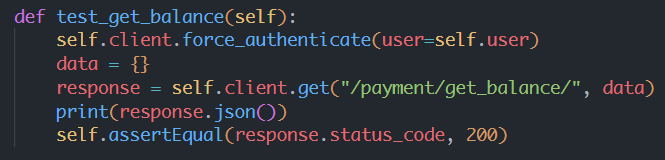
\includegraphics[scale=0.7]{unit_testing_codes/get_balance.png}
\end{center}

\subsubsection{Updating Wallet Balance}
\textbf{API Endpoint: } \texttt{/payment/update\_balance/} \\
\textbf{Test Owner: } Ananya Baghel \\
\textbf{Date: } 28/03/2024 \\
\textbf{Test Description: } This test case is used to check if a user can update their wallet balance. \\
\textbf{Test Results: } User is able to update their wallet balance successfully.\\

\begin{center}
    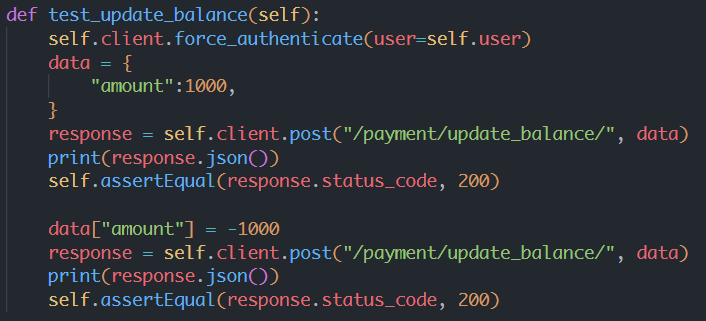
\includegraphics[scale=0.7]{unit_testing_codes/update_balance.png}
\end{center}

\subsubsection{Viewing Transaction History}
\textbf{API Endpoint: } \texttt{/payment/get\_transactions/} \\
\textbf{Test Owner: } Ananya Baghel \\
\textbf{Date: } 28/03/2024 \\
\textbf{Test Description: } This test case is used to check if a user can view their transaction history. \\
\textbf{Test Results: } User is able to view their transaction history successfully.\\

\begin{center}
    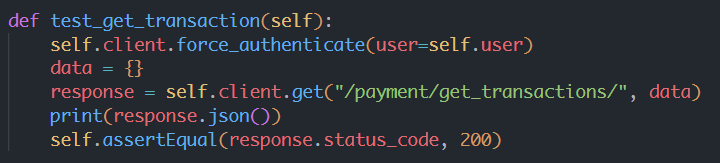
\includegraphics[scale=0.8]{unit_testing_codes/transaction_history.png}
\end{center}

\appendixpageoff
\begin{appendices}

\newpage

\section{\centering{\textbf{Group Log}}}
\begin{tabular}{|p{1cm}|p{2cm}|p{2cm}|p{2cm}|p{6.75cm}|}
\hline
\makecell{\textbf{S.No}} & \makecell{\textbf{Date}} & \makecell{\textbf{Timings}} & \makecell{\textbf{Venue}} & \makecell{\textbf{Description}} \\
\hline
\makecell{1} & \makecell{07/01/2024} & \makecell{14:00\\ to \\16:00} & \makecell{RM \\Building} & \makecell{Brain-stormed various possible \\ prospective ideas for the project. \\ Main ideas presented were: \\ Bicycle Rental Services \\ Hall Management \\ Used goods Buy/Sell Portal} \\
\hline
\makecell{2} & \makecell{09/01/2024} & \makecell{14:30\\to\\17:00} & \makecell{Google\\ Meet} & \makecell{Finalized the idea for the project and \\ discussed various aspects of it.} \\
\hline
\makecell{3} & \makecell{11/01/2024} & \makecell{22:00\\to\\00:00} & \makecell{Google\\Meet} & \makecell{Studied the SRS template given and \\ distributed the work amongst the team \\ members.} \\
\hline
\makecell{4} & \makecell{17/01/2024} & \makecell{21:00\\to\\21:30} & \makecell{Google\\Meet} & \makecell{First meet with the Teaching Assistant \\ Mr. Bharat. Discussed about project \\ and the SRS documentation.} \\
\hline
\makecell{5} & \makecell{20/01/2024} & \makecell{15:00\\to\\18:00} & \makecell{Google\\Meet} & \makecell{Brainstorming of final ideas and \\ discussion on use cases, features, \\ data flows.} \\
\hline
\makecell{6} & \makecell{21/01/2024} & \makecell{14:00\\to\\15:00} & \makecell{Google\\Meet} & \makecell{Decided to use Django with bootstrap \\ and inline CSS to build the front end \\ part of our application and PostgreSQL \\ as our DBMS.} \\
\hline
\makecell{7} & \makecell{22/01/2024} & \makecell{23:00\\to\\00:00} & \makecell{Google\\Meet} & \makecell{Explored more functionalities for the \\ product and progressed with the SRS \\ document.} \\
\hline
\makecell{8} & \makecell{25/01/2024} & \makecell{14:00\\to\\17:00} & \makecell{RM\\Building} & \makecell{Finalized the SRS Document and\\completed typesetting in \LaTeX} \\
\hline
\end{tabular}
\end{appendices}
\end{document}
